\subsection*{e)}
Here we will investigate the mixing and the posteriors in the proposal distribution. From the relation of $R$ in the definition. We note that $R$ depends both on $\rho$ and $t_{i+1}-t_{i-1}$. One can realize first that $R$ will be calculated for each breakpoint, hence an increase of breakpoints used, a decrease of the value of the differences will occur. We therefore need to increase $\rho$ accordingly. \\
\\
We know that $\rho$ will effect our sample space. Therefore if we choose $\rho$ for values 
\[ || \rho || > 0 + C, \quad \text{for} \quad C>> 0 \] 
indicates that we will consider a large portion of the sample space, in our case $X\in\mathbb{R}$. This in turn will only generate rejected samples, since we are almost 100\% outside of the our desired sample space. However, if $\rho=0$ or close to $0$, 
\[ || \rho ||+ \epsilon \geq 0,  \quad \text{for} \quad \epsilon \geq 0 \] 
we do not sample outside of the proposed distribution, meaning that we will only end up in the proposed values and again reject most of the sampled values. \\
\\
We know that $\rho$ must help to enclose the desired sample space. Since we know from the argumentation above, $\rho$ must be small and large enough but also depend on the breakpoints. Below in figures \ref{fig:fixrho1} and \ref{fig:fixrho4} are plots of the mixing for $\boldsymbol{t}$ with a fixed $\rho$. \\
\\
\begin{figure}[H]
  \centering
\begin{minipage}{1\textwidth}
    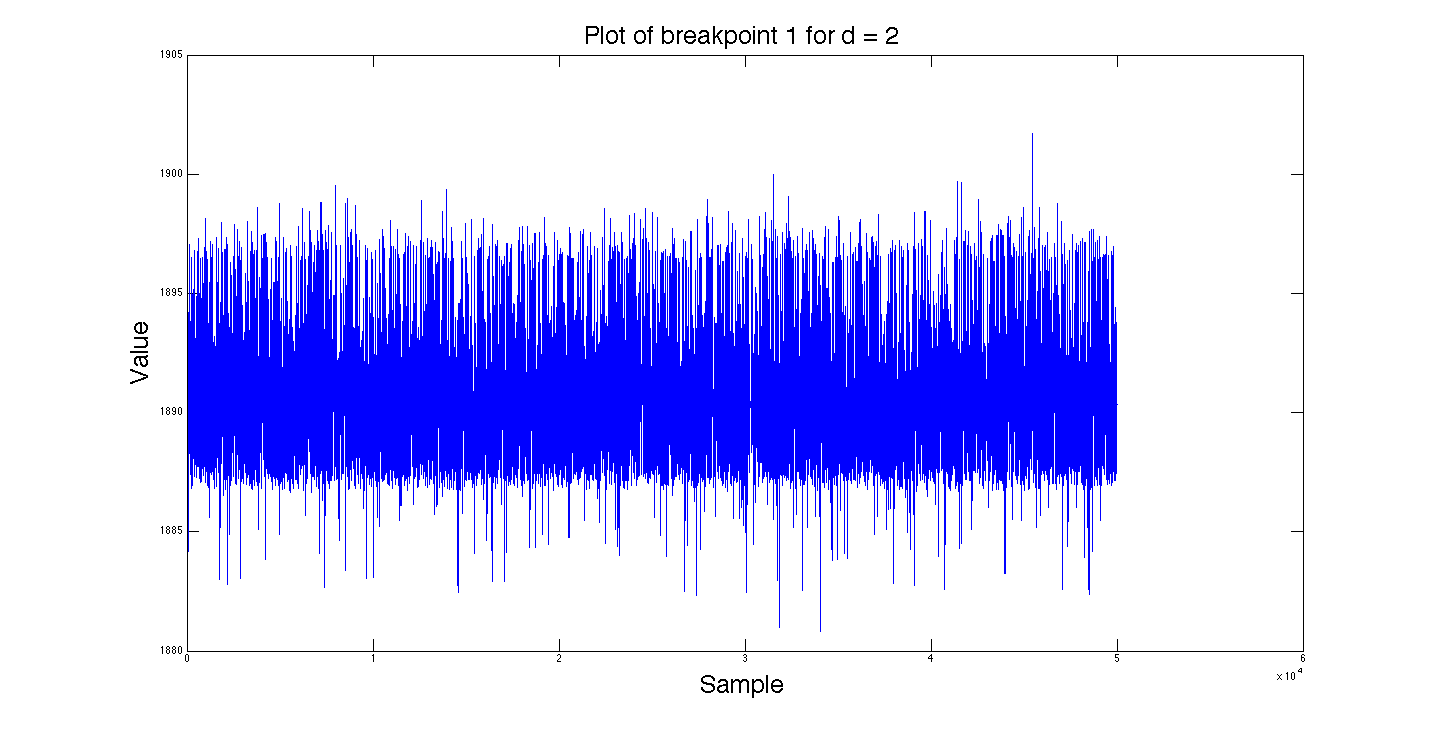
\includegraphics[scale=0.28]{./Figures/fixrho1.png}
  \label{fig:fixrho1}
\end{minipage}
%
\begin{minipage}{1\textwidth}
    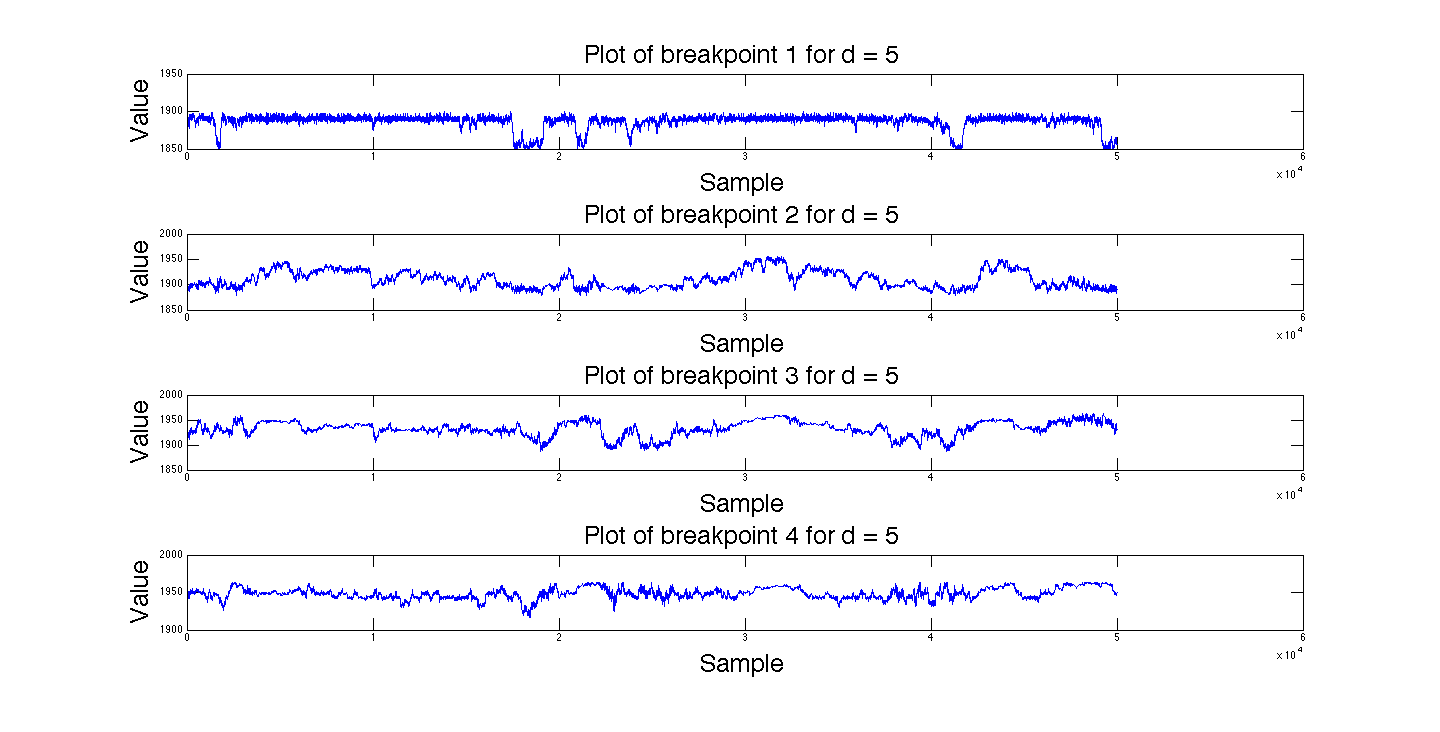
\includegraphics[scale=0.28]{./Figures/fixrho4.png}
  \label{fig:fixrho4}
\end{minipage}

  \caption[An Electron]{Figure of t-posterior for one and four breakpoints for a fixed constant $\rho=0.05$}
\end{figure}

One can deduce from the figures \ref{fig:fixrho1},\ref{fig:fixrho4} that the mixing is good for one breakpoint. However, we will have more correlated values when using $\rho=0.05$ for four breakpoints. Instead of using a constant $\rho$ we introduce a varing $\rho$ which is determined by the number of breakpoints used.

\begin{figure}[H]

  \centering
\begin{minipage}{1\textwidth}
    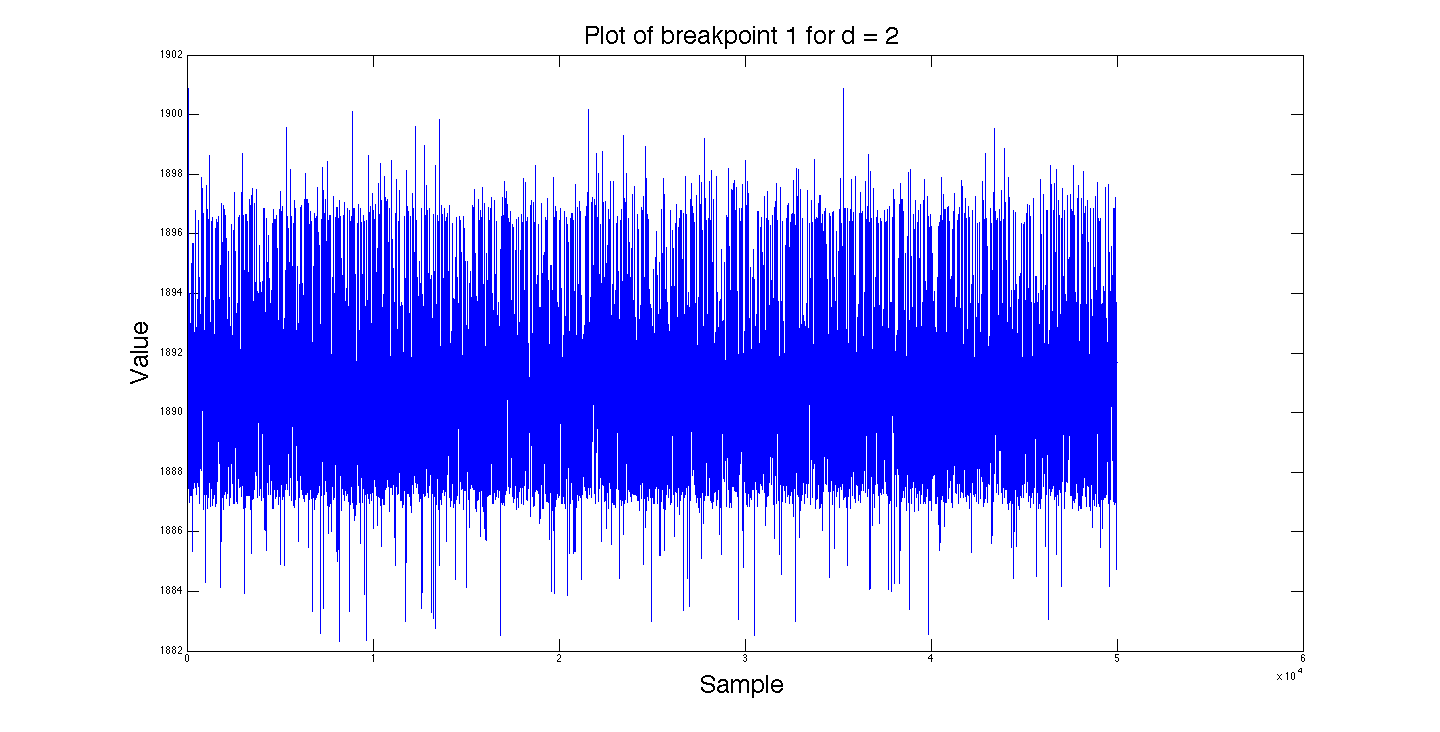
\includegraphics[scale=0.28]{./Figures/varrho1.png}
  \label{fig:varrho1}
\end{minipage}

\begin{minipage}{1\textwidth}
    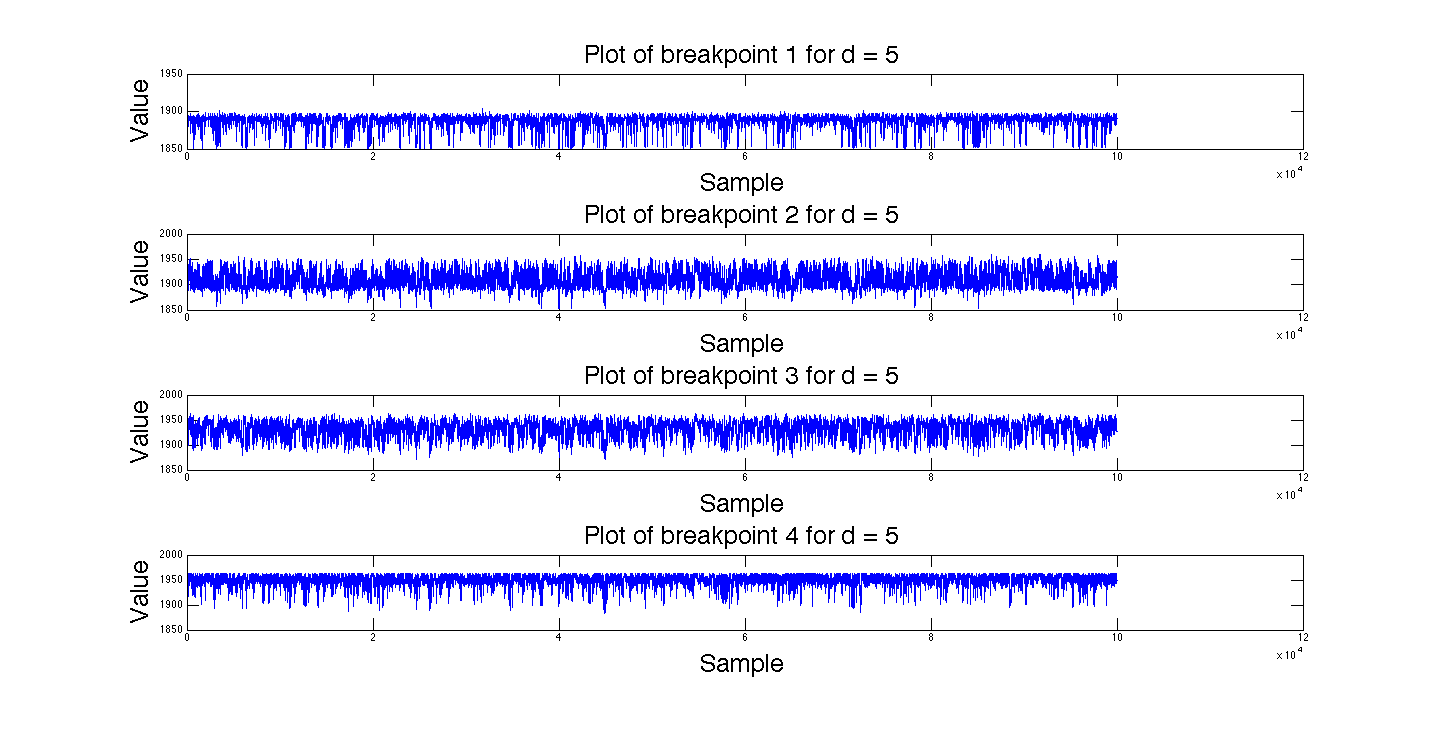
\includegraphics[scale=0.28]{./Figures/t4.png}
  \label{fig:varrho4}
\end{minipage}

  \caption[An Electron]{Figure of t-posterior for breakpoints$=1,4$ for a varing $\rho$}
\end{figure}

From the figures \ref{fig:varrho1},\ref{fig:varrho4} one can see that the mixing is more random and non-correlated compared with the fixed $\rho$. Indicating that our values should be better approximated using this relation.
